\documentclass{report}
\usepackage{listings}
\usepackage{graphicx}

\title{Report on CNN/Scattering classification comparison}
\author{Alberto Carli \and Gabriele Roncolato \and Leonardo Zecchin }
\date{}

\begin{document}
\maketitle
\tableofcontents
\pagebreak

\chapter{Introduction}
This document illustrates the project valid for the Visual Intelligence class of the academic year 2022/2023. \\
The assignment tests the knowledge gained in class by applying signal analysis methods, in particular we classified signals by using \textbf{Convolutional Neural Networks} and wavelet theory, specifically  \textbf{Wavelet Scattering}. \\
In this project we implemented the code necessary to classify a given dataset first by training and testing a CNN, then by applying the Wavelet Scattering Transform and training a NN with the extracted features.
Finally we compared the results obtained with these two methods in terms of accuracy against how many epochs were used to train the classifiers. \\
For the entire project, we followed the guidelines given during the laboratory lectures.


\chapter{Dataset}
We employed a dataset consisting of 128x128 RGB images divided into two categories: dogs and flowers. There are 1600 pictures of single dogs and 1387 pictures of single flowers.
70\% of the dataset is used for training, while the remaining 30\% is allocated for running tests with the classifiers.

\chapter{Objectives}
The goal of this project is to explore the use of scattering transforms to improve the performance of neural networks on a given dataset.\\
Specifically, we aimed to compare the performance of a CNN trained on the original dataset to a NN trained on the scattering decomposition of the data.\\

We then visualized the filters learned by the CNN and compared them to the ones applied by the scattering transform to gain insight into the types of features that were extracted. 
By accomplishing these objectives we hoped to gain a better understanding of how the CNN learns which features to extract.

\chapter{CNN Classification}
\section{What is a CNN}
A Convolutional Neural Network (\textbf{CNN}) is a type of deep learning algorithm commonly used for image recognition and computer vision tasks. It is designed to automatically learn and extract relevant features from input images through convolutional and pooling layers, followed by fully connected layers that produce output predictions. \\
The \texttt{CNN\_128x128} architecture consists of four \textbf{convolutional} layers and three fully connected layers. The first layer takes an input image with \texttt{input\_channel} number of channels, and the output of the last layer is a vector with \texttt{num\_classes} elements representing the probability of each class.

\section{Architecture}


\begin{lstlisting}[language=bash]
CNN_128x128(
  (conv1): Conv2d(3, 32, kernel_size=(9, 9), stride=(1, 1))
  (conv2): Conv2d(32, 32, kernel_size=(9, 9), stride=(1, 1))
  (conv3): Conv2d(32, 64, kernel_size=(5, 5), stride=(1, 1))
  (conv4): Conv2d(64, 64, kernel_size=(5, 5), stride=(1, 1))
  (drop1): Dropout1d(p=0.1, inplace=False)
  (flat): Flatten(start_dim=1, end_dim=-1)
  (fc1): Linear(in_features=576, out_features=256, bias=True)
  (drop2): Dropout(p=0.1, inplace=False)
  (fc2): Linear(in_features=256, out_features=32, bias=True)
  (fc3): Linear(in_features=32, out_features=2, bias=True)
)
\end{lstlisting}


\subsection{Convolutional Layers}

The first convolutional layer has 32 output channels, while the second convolutional layer has 64 output channels. The third and fourth convolutional layers also have 64 output channels, but they use a smaller kernel size of 5x5 instead of 9x9 used in the first two layers. All convolutional layers have a stride of 1 and use a \textbf{Rectified Linear Unit} (\textbf{ReLU}) activation function.
\subsection{Dropout}

The dropout layer is used to prevent overfitting in the model. In this architecture, we use a dropout rate of 0.1.
\subsection{Flatten Layer}

The flatten layer is used to convert the output of the last convolutional layer into a vector (\textit{tensor}), which can be used as input for the fully connected layers. In this architecture the flatten layer converts the output of the last convolutional layer into a vector of size 576.

\subsection{Fully Connected Layers}
The fully connected layers consist of three layers, with 256, 32 and \texttt{num\_classes} neurons respectively. All fully connected layers use a ReLU activation function except for the last layer, which uses the \textbf{softmax function} to output the class probabilities.

\section{Training the Model}

To train the model, we pass the input images through the CNN and compute the loss function (in this case \textbf{cross-entropy}) between the predicted class probabilities and the true labels. We use \textbf{stochastic gradient descent} to optimize the model weights, with a \textit{learning rate} of 0.001 and a \textit{momentum} of 0.9. The model is trained for a fixed number of epochs, and the best model is selected based on its performance on a validation set.

\chapter{Scattering+NN Classification}
\section{Wavelet Scattering}
For the scattering part, we used the \texttt{kymatio} library and in particular we used the function \texttt{Scattering2D} which computes the 2D wavelet scattering transform of an input image, with a specified number of scales, maximum scattering order, and number of rotations. \\
The output of the Scattering2D function is a multi-dimensional PyTorch tensor containing the wavelet scattering coefficients of the input image.
We found the best results with the following values:
\begin{itemize}
    \item \texttt{J} = ...: parameter represents the number of scales to use in the wavelet transform .
    \item \texttt{order} = ...: is the maximum order of wavelet scattering coefficients to compute .
    \item $\texttt{L} = ...$: specifies the number of rotations to use in the wavelet transform .
\end{itemize}
\section{Neural Network}
The \texttt{NN\_128x128} class defines a Neural Network (NN) for classification tasks. The network expects input with a specified number of channels, \texttt{input\_channel}, and the number of output classes, \texttt{num\_classes}. The class inherits from the \texttt{nn.Module} class, which is a base class for all neural network modules in PyTorch.

\subsection{Architecture}
The NN architecture defined in the NN\_128x128 class consists of only \textbf{fully connected layers}. There are no convolutional layers that are typically used in a CNN. Instead, the data is flattened using the \texttt{nn.Flatten()} layer and passed to the fully connected layers.

The architecture of the network consists of three fully connected layers. The first layer, \texttt{self.fc1}, has 256 output neurons, and the input size is 243. The second layer, \texttt{self.fc2}, has 32 output neurons, and the third and final layer, \texttt{self.fc3}, has \texttt{num\_classes} output neurons.

Between the second and third layer, there is a dropout layer, \texttt{self.drop2}, with a dropout rate of 0.1. The dropout layer helps to prevent overfitting of the model.

The activation function used in the network is \textbf{ReLU}, which is applied after each fully connected layer. The last layer uses the \textbf{softmax} function to produce probabilities for each of the \texttt{num\_classes} output neurons. 

\chapter{Performances comparison}
After some parameters tuning, we found that the best results were obtained with the following parameters:
\begin{itemize}
    \item \texttt{J} = 3: parameter represents the number of scales to use in the wavelet transform .
    \item \texttt{order} = 2: is the maximum order of wavelet scattering coefficients to compute .
    \item $\texttt{L} = 8$: specifies the number of rotations to use in the wavelet transform .
\end{itemize}
we tried optimizing the scattering transform to try and reach the CNN's performances.\\
We tried different scales (J) and rotations (L) and we found that \\
We tried different trainset sizes and we found that \\
We tried different number of epochs and we found that \\
(\textbf{Da Controllare da qui in poi.})\\
In this chapter we are going to compare the results obtained with \textbf{CNN} and \textbf{wavelet scattering}.\\
We tried different values for the following parameters:
\begin{itemize}
    \item \texttt{batch size}, the number of samples used in one iteration to update the model's weights;
    \item \texttt{learning rate}, controls the speed of weight updates during training;
    \item \texttt{momentum}, scale for past experience to not be perturbated by new ones;
    \item \texttt{epochs}, the number of times the model is trained on the entire training dataset;
    \item \texttt{invariance scale}, specifies the spatial support in the row and column dimensions of the scaling filter;
    \item \texttt{rotations}, number of rotations per wavelet per filter bank in the scattering network;
    \item \texttt{quality factor}, the quality factor is the number of wavelet filters per octave;
    \item \texttt{training datasize}, the number of images used.
\end{itemize}
To influence the results of CNN we modified these parameters: batch size, learning rate, momentum, epochs and the training datasize and to influence the results of the wavelet scattering + NN we modified these parameters: invariance scale, rotations, quality factor.\\
We found that the best results for the CNN were obtained with the following parameters:
\begin{itemize}
    \item \texttt{batch size = 64}
    \item \texttt{learning rate = 0.001}
    \item \texttt{momentum = 0.5}
    \item \texttt{epochs = 100}
    \item \texttt{training datasize = 500}
\end{itemize}
and the best results for the wavelet scattering + NN were obtained with:
\begin{itemize}
    \item \texttt{invariance scale = 5}
    \item \texttt{rotations =  [8,8]};
    \item \texttt{quality factor = [2,1]}
\end{itemize}
\textbf{CNN metrics}: \\
Accuracy:               0.82\\
Precision:              0.875\\
Recall:                 0.7777777777777778\\
F1:                     0.823529411764706\\
\textbf{NN metrics}:\\
Accuracy:               0.87\\
Precision:              0.9019607843137255\\
Recall:                 0.8518518518518519\\
F1:                             0.8761904761904761\\
\begin{figure}
    \centering
    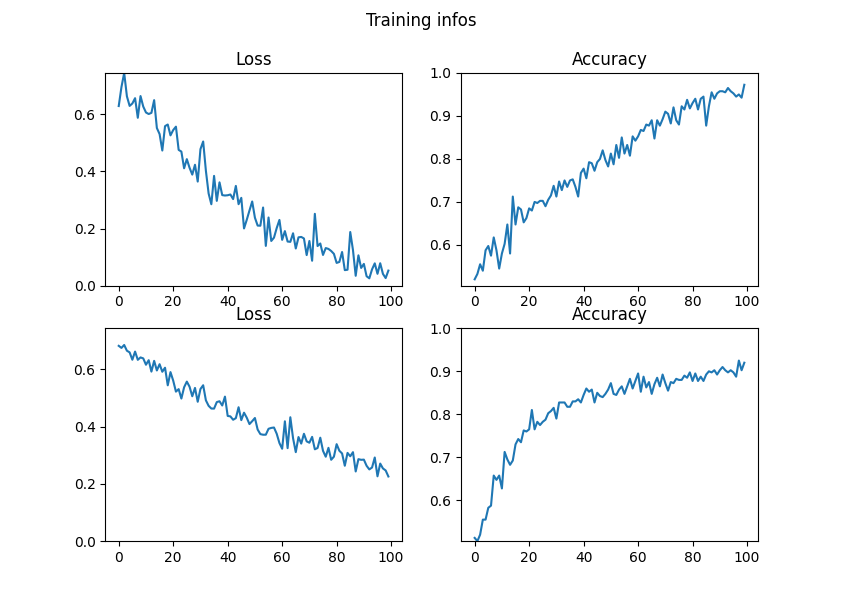
\includegraphics[width=8cm]{images/0.82/training_infos.png}\hfill
    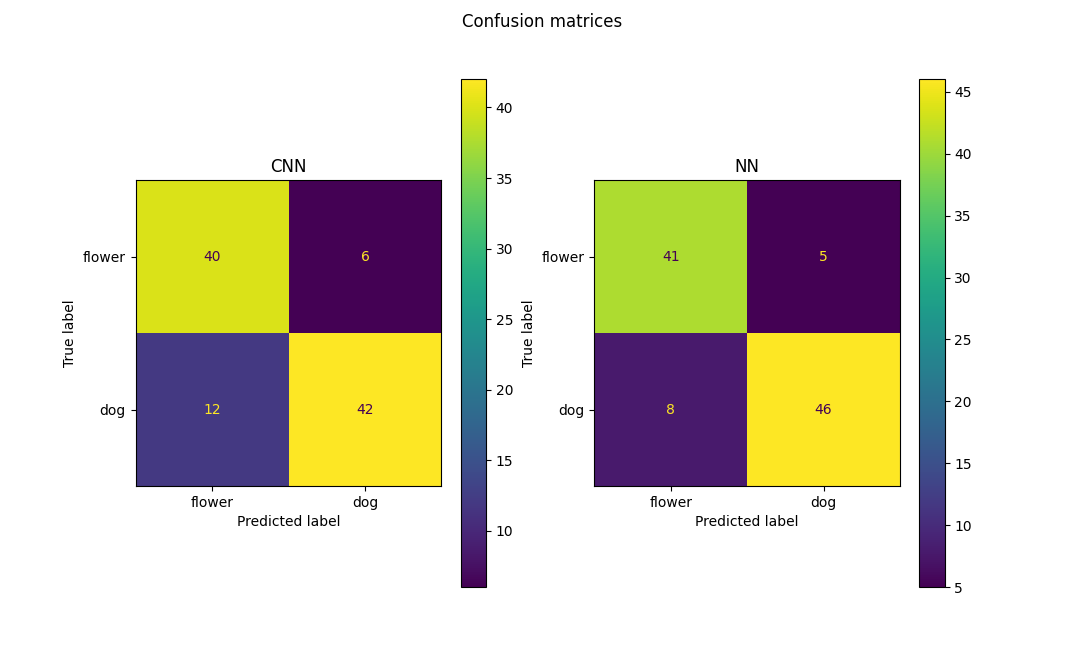
\includegraphics[width=8cm]{images/0.82/conf_mat.png}\hfill
    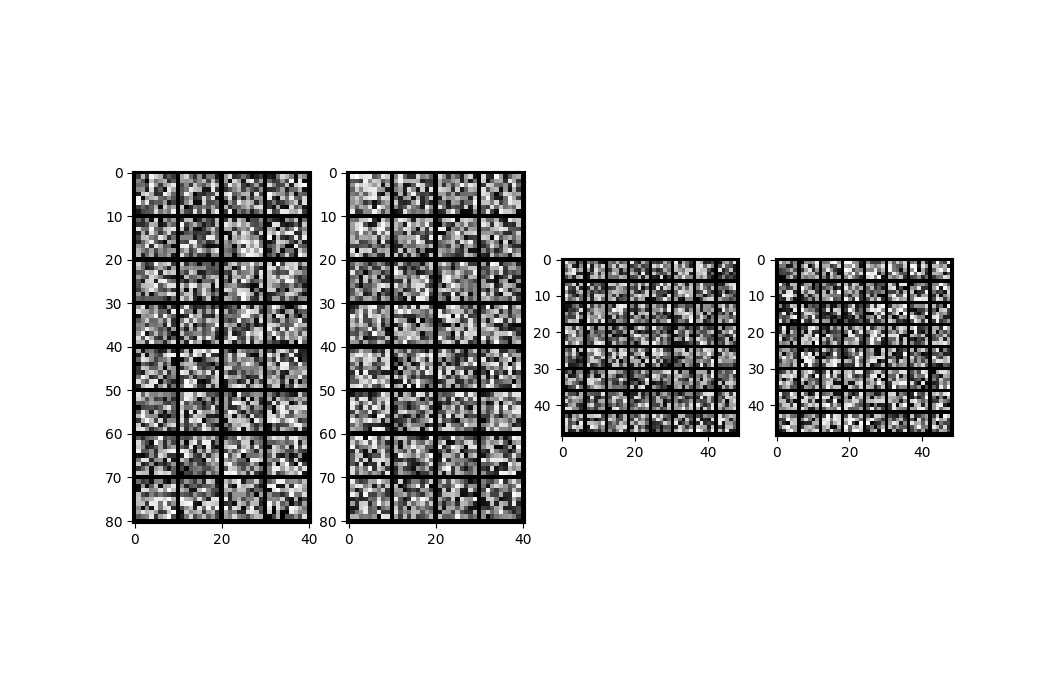
\includegraphics[width=8cm]{images/0.82/cnn_filters.png}
    \caption{First run}
    \label{fig:my_label}
\end{figure}

\chapter{Filters}
\chapter{Conclusions}
\end{document}




